%%%%%%%%%%%%%%%%%%%%%%%%%%%%%%%%%%%%%%%%%%%%%%%%%%%%%%%%%%%%
% 1.7 GALOIS THEORY
% The Composition of Advanced Mathematics
%%%%%%%%%%%%%%%%%%%%%%%%%%%%%%%%%%%%%%%%%%%%%%%%%%%%%%%%%%%%

\section{Galois Theory}
\label{sec:galois-theory}

\prerequisite{
Functions from \cref{sec:functions}, methods of proof from
\cref{sec:methods-of-proof}, group theory from \cref{sec:group-theory},
ring theory from \cref{sec:ring-theory}, and especially field theory from
\cref{sec:field-theory}.
}

\learningobjectives{
By the end of this section, the reader should be able to:
\begin{itemize}
    \item explain the central problem and philosophy of Galois theory;
    \item identify field automorphisms that fix a base field;
    \item define the Galois group of a field extension;
    \item determine elementary Galois groups;
    \item distinguish normal, separable, and Galois extensions;
    \item interpret conjugate elements through field embeddings;
    \item relate polynomial roots to field automorphisms;
    \item compute fixed fields in elementary examples;
    \item state and apply the Fundamental Theorem of Galois Theory;
    \item translate between intermediate fields and subgroups;
    \item understand the reversal of inclusion in the Galois correspondence;
    \item recognize the significance of normal subgroups;
    \item relate quotient groups to intermediate extensions;
    \item understand the connection between solvable groups and solvability by radicals;
    \item explain why no general radical formula exists for polynomial equations of degree five or greater.
\end{itemize}
}

%%%%%%%%%%%%%%%%%%%%%%%%%%%%%%%%%%%%%%%%%%%%%%%%%%%%%%%%%%%%
\subsection{From Polynomial Equations to Symmetry}
\label{subsec:galois-polynomial-symmetry}
%%%%%%%%%%%%%%%%%%%%%%%%%%%%%%%%%%%%%%%%%%%%%%%%%%%%%%%%%%%%

Field theory asks how a field can be enlarged so that a polynomial acquires
its missing roots.

Galois theory asks a deeper question:

\begin{center}
\emph{What symmetries exist among those roots?}
\end{center}

Consider

\[ f(x)=x^2-2. \]

Its roots are

\[ \sqrt2\qquad\text{and}\qquad-\sqrt2. \]

The splitting field over \(\Q\) is

\[ \Q(\sqrt2). \]

There is a nontrivial field automorphism

\[ \sigma:\Q(\sqrt2)\to\Q(\sqrt2) \]

defined by

\[ \sigma(a+b\sqrt2)=a-b\sqrt2. \]

It fixes every rational number while exchanging the two roots:

\[ \sqrt2\longleftrightarrow-\sqrt2. \]

This is the basic idea of Galois theory.

\begin{conceptbox}
Galois theory studies polynomial equations by studying the symmetry group of
their roots.

The bridge is

\[ \boxed{\text{polynomials}\longleftrightarrow\text{fields}\longleftrightarrow\text{groups}}. \]
\end{conceptbox}

%%%%%%%%%%%%%%%%%%%%%%%%%%%%%%%%%%%%%%%%%%%%%%%%%%%%%%%%%%%%
\subsection{The Galois Theory Bridge}
\label{subsec:galois-bridge}
%%%%%%%%%%%%%%%%%%%%%%%%%%%%%%%%%%%%%%%%%%%%%%%%%%%%%%%%%%%%

The main structures fit together schematically as follows.

\begin{center}
\begin{tikzpicture}[
    node distance=16mm and 18mm,
    box/.style={draw,rounded corners,align=center,inner sep=6pt},
    >=stealth
]
\node[box] (poly) {Polynomial\\\(f(x)\in K[x]\)};
\node[box,right=of poly] (field) {Splitting field\\\(L/K\)};
\node[box,right=of field] (group) {Symmetry group\\\(\Gal(L/K)\)};

\draw[->,thick] (poly)--node[above]{adjoin roots}(field);
\draw[->,thick] (field)--node[above]{automorphisms}(group);
\draw[<->,thick,bend right=30] (poly) to node[below]{root structure} (group);
\end{tikzpicture}
\end{center}

The remarkable feature is that information about a polynomial can be encoded
inside a finite group.

%%%%%%%%%%%%%%%%%%%%%%%%%%%%%%%%%%%%%%%%%%%%%%%%%%%%%%%%%%%%
\subsection{Automorphisms Fixing a Base Field}
\label{subsec:automorphisms-fixing-field}
%%%%%%%%%%%%%%%%%%%%%%%%%%%%%%%%%%%%%%%%%%%%%%%%%%%%%%%%%%%%

Suppose

\[ K\subseteq L. \]

A field automorphism of \(L\) need not preserve every element individually.

Galois theory focuses on automorphisms that leave the base field \(K\)
unchanged.

\begin{definitionbox}{Automorphism Fixing a Field}
Let \(L/K\) be a field extension. An automorphism
\[ \sigma:L\to L \]
\emph{fixes \(K\)} if
\[ \sigma(a)=a \]
for every \(a\in K\).
\end{definitionbox}

Such an automorphism is also called a \(K\)-automorphism of \(L\).

%%%%%%%%%%%%%%%%%%%%%%%%%%%%%%%%%%%%%%%%%%%%%%%%%%%%%%%%%%%%
\subsection{The Galois Group}
\label{subsec:galois-group}
%%%%%%%%%%%%%%%%%%%%%%%%%%%%%%%%%%%%%%%%%%%%%%%%%%%%%%%%%%%%

\begin{definitionbox}{Galois Group}
Let \(L/K\) be a field extension. The \emph{Galois group} of \(L\) over \(K\)
is the group of all field automorphisms of \(L\) that fix \(K\):
\[ \Gal(L/K)=\{\sigma\in\operatorname{Aut}(L):\sigma(a)=a\text{ for every }a\in K\}. \]
\end{definitionbox}

The notation

\[ \Gal(L/K) \]

is read ``the Galois group of \(L\) over \(K\).''

The operation in this group is function composition.

%%%%%%%%%%%%%%%%%%%%%%%%%%%%%%%%%%%%%%%%%%%%%%%%%%%%%%%%%%%%
\subsection{Why the Galois Automorphisms Form a Group}
\label{subsec:galois-automorphisms-group}
%%%%%%%%%%%%%%%%%%%%%%%%%%%%%%%%%%%%%%%%%%%%%%%%%%%%%%%%%%%%

The set \(\Gal(L/K)\) forms a group because:

\begin{itemize}
    \item the composition of two automorphisms fixing \(K\) also fixes \(K\);
    \item composition of functions is associative;
    \item the identity map fixes \(K\);
    \item the inverse of an automorphism fixing \(K\) also fixes \(K\).
\end{itemize}

Thus

\[ \Gal(L/K)\leq\operatorname{Aut}(L). \]

%%%%%%%%%%%%%%%%%%%%%%%%%%%%%%%%%%%%%%%%%%%%%%%%%%%%%%%%%%%%
\subsection{First Example: \(\Q(\sqrt2)/\Q\)}
\label{subsec:galois-q-sqrt2}
%%%%%%%%%%%%%%%%%%%%%%%%%%%%%%%%%%%%%%%%%%%%%%%%%%%%%%%%%%%%

Every element of \(\Q(\sqrt2)\) has the form

\[ a+b\sqrt2,\qquad a,b\in\Q. \]

An automorphism fixing \(\Q\) must send \(\sqrt2\) to another root of its
minimal polynomial

\[ x^2-2. \]

Therefore,

\[ \sqrt2\mapsto\sqrt2 \]

or

\[ \sqrt2\mapsto-\sqrt2. \]

Hence there are exactly two automorphisms.

The identity is

\[ e(a+b\sqrt2)=a+b\sqrt2. \]

The nontrivial automorphism is

\[ \sigma(a+b\sqrt2)=a-b\sqrt2. \]

Therefore,

\[ \Gal(\Q(\sqrt2)/\Q)=\{e,\sigma\}. \]

Since

\[ \sigma^2=e, \]

we have

\[ \Gal(\Q(\sqrt2)/\Q)\cong C_2. \]

%%%%%%%%%%%%%%%%%%%%%%%%%%%%%%%%%%%%%%%%%%%%%%%%%%%%%%%%%%%%
\subsection{Visualizing the First Galois Group}
\label{subsec:visual-first-galois-group}
%%%%%%%%%%%%%%%%%%%%%%%%%%%%%%%%%%%%%%%%%%%%%%%%%%%%%%%%%%%%

\begin{center}
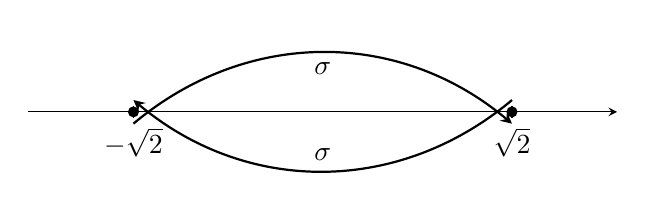
\begin{tikzpicture}[x=1.7cm,>=stealth]
\draw[->] (-2.2,0)--(2.2,0);

\draw (-1.414,0.08)--(-1.414,-0.08);
\draw (1.414,0.08)--(1.414,-0.08);

\node[below] at (-1.414,-0.08) {\(-\sqrt2\)};
\node[below] at (1.414,-0.08) {\(\sqrt2\)};

\fill (-1.414,0) circle (2pt);
\fill (1.414,0) circle (2pt);

\draw[->,thick,bend left=40]
    (1.414,0.15) to node[above]{\(\sigma\)} (-1.414,0.15);

\draw[->,thick,bend left=40]
    (-1.414,-0.15) to node[below]{\(\sigma\)} (1.414,-0.15);
\end{tikzpicture}
\end{center}

The nontrivial symmetry simply exchanges the two roots.

%%%%%%%%%%%%%%%%%%%%%%%%%%%%%%%%%%%%%%%%%%%%%%%%%%%%%%%%%%%%
\subsection{Why Automorphisms Permute Roots}
\label{subsec:automorphisms-permute-roots}
%%%%%%%%%%%%%%%%%%%%%%%%%%%%%%%%%%%%%%%%%%%%%%%%%%%%%%%%%%%%

Suppose

\[ f(x)\in K[x] \]

and

\[ \sigma\in\Gal(L/K). \]

If

\[ f(\alpha)=0, \]

then

\[ f(\sigma(\alpha))=0. \]

To see why, write

\[ f(x)=a_0+a_1x+\cdots+a_nx^n, \qquad a_i\in K. \]

Since \(\sigma\) fixes every coefficient,

\[
\begin{aligned}
0
&=\sigma(f(\alpha))\\
&=\sigma(a_0+a_1\alpha+\cdots+a_n\alpha^n)\\
&=a_0+a_1\sigma(\alpha)+\cdots+a_n\sigma(\alpha)^n\\
&=f(\sigma(\alpha)).
\end{aligned}
\]

Therefore Galois automorphisms send roots to roots of the same polynomial.

\begin{importantbox}
Galois automorphisms do not arbitrarily move elements.

They must preserve every algebraic relation whose coefficients lie in the
base field.
\end{importantbox}

%%%%%%%%%%%%%%%%%%%%%%%%%%%%%%%%%%%%%%%%%%%%%%%%%%%%%%%%%%%%
\subsection{Root Permutations}
\label{subsec:galois-root-permutations}
%%%%%%%%%%%%%%%%%%%%%%%%%%%%%%%%%%%%%%%%%%%%%%%%%%%%%%%%%%%%

Suppose a polynomial splits in \(L\) as

\[ f(x)=a(x-\alpha_1)(x-\alpha_2)\cdots(x-\alpha_n). \]

Every element of \(\Gal(L/K)\) permutes the roots

\[ \alpha_1,\alpha_2,\ldots,\alpha_n. \]

Therefore the Galois group can often be represented as a subgroup of the
symmetric group

\[ S_n. \]

This provides the direct connection between field theory and permutation
groups.

%%%%%%%%%%%%%%%%%%%%%%%%%%%%%%%%%%%%%%%%%%%%%%%%%%%%%%%%%%%%
\subsection{A Root-Permutation Diagram}
\label{subsec:galois-root-permutation-diagram}
%%%%%%%%%%%%%%%%%%%%%%%%%%%%%%%%%%%%%%%%%%%%%%%%%%%%%%%%%%%%

\begin{center}
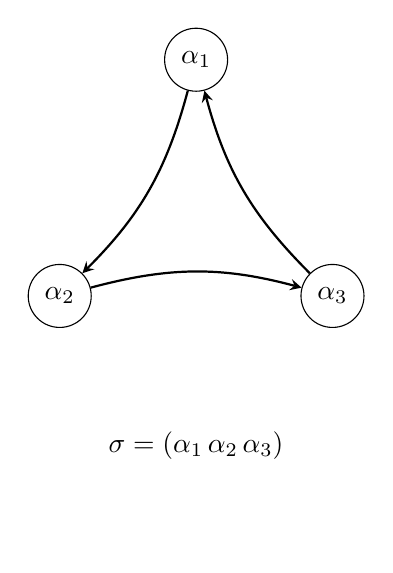
\begin{tikzpicture}[
    every node/.style={circle,draw,minimum size=8mm},
    >=stealth
]
\node (a1) at (90:2) {\(\alpha_1\)};
\node (a2) at (210:2) {\(\alpha_2\)};
\node (a3) at (330:2) {\(\alpha_3\)};

\draw[->,thick,bend left=15] (a1) to (a2);
\draw[->,thick,bend left=15] (a2) to (a3);
\draw[->,thick,bend left=15] (a3) to (a1);

\node[draw=none] at (0,-2.9) {\(\sigma=(\alpha_1\,\alpha_2\,\alpha_3)\)};
\end{tikzpicture}
\end{center}

A field automorphism may therefore be studied through its permutation action
on polynomial roots.

%%%%%%%%%%%%%%%%%%%%%%%%%%%%%%%%%%%%%%%%%%%%%%%%%%%%%%%%%%%%
\subsection{Conjugate Elements}
\label{subsec:galois-conjugates}
%%%%%%%%%%%%%%%%%%%%%%%%%%%%%%%%%%%%%%%%%%%%%%%%%%%%%%%%%%%%

Elements sharing the same minimal polynomial over a base field are closely
related.

\begin{definitionbox}{Conjugates over a Field}
Let \(\alpha\) be algebraic over \(K\). The roots of the minimal polynomial
\[ m_{\alpha,K}(x) \]
are called the \emph{conjugates of \(\alpha\) over \(K\)}.
\end{definitionbox}

For example, the conjugates of \(\sqrt2\) over \(\Q\) are

\[ \sqrt2\qquad\text{and}\qquad-\sqrt2. \]

The conjugates of \(i\) over \(\R\) are

\[ i\qquad\text{and}\qquad-i. \]

%%%%%%%%%%%%%%%%%%%%%%%%%%%%%%%%%%%%%%%%%%%%%%%%%%%%%%%%%%%%
\subsection{Embeddings and Conjugates}
\label{subsec:embeddings-conjugates}
%%%%%%%%%%%%%%%%%%%%%%%%%%%%%%%%%%%%%%%%%%%%%%%%%%%%%%%%%%%%

Suppose

\[ K(\alpha)/K \]

is an algebraic extension.

A \(K\)-embedding

\[ \sigma:K(\alpha)\to L \]

is determined by the image of \(\alpha\).

Because \(\sigma(\alpha)\) must satisfy the same minimal polynomial as
\(\alpha\), it must be one of the conjugates of \(\alpha\).

Thus the possible embeddings of a simple algebraic extension are closely
related to the roots of the minimal polynomial.

%%%%%%%%%%%%%%%%%%%%%%%%%%%%%%%%%%%%%%%%%%%%%%%%%%%%%%%%%%%%
\subsection{Separable Polynomials}
\label{subsec:separable-polynomials}
%%%%%%%%%%%%%%%%%%%%%%%%%%%%%%%%%%%%%%%%%%%%%%%%%%%%%%%%%%%%

The number of distinct roots matters in Galois theory.

\begin{definitionbox}{Separable Polynomial}
A polynomial \(f(x)\in K[x]\) is \emph{separable over \(K\)} if it has no
repeated roots in a splitting field.
\end{definitionbox}

For example,

\[ x^2-2 \]

has two distinct roots

\[ \sqrt2,\qquad-\sqrt2, \]

so it is separable over \(\Q\).

%%%%%%%%%%%%%%%%%%%%%%%%%%%%%%%%%%%%%%%%%%%%%%%%%%%%%%%%%%%%
\subsection{Repeated Roots and the Formal Derivative}
\label{subsec:repeated-roots-derivative}
%%%%%%%%%%%%%%%%%%%%%%%%%%%%%%%%%%%%%%%%%%%%%%%%%%%%%%%%%%%%

Repeated roots can be detected algebraically.

Let

\[ f(x)\in K[x]. \]

Its formal derivative is denoted

\[ f'(x). \]

A polynomial has a repeated root in a splitting field precisely when

\[ \gcd(f,f')\neq1. \]

Therefore,

\[ f\text{ is separable}\iff\gcd(f,f')=1. \]

This criterion uses the algebraic derivative of a polynomial and does not
require analytic limits.

%%%%%%%%%%%%%%%%%%%%%%%%%%%%%%%%%%%%%%%%%%%%%%%%%%%%%%%%%%%%
\subsection{Example of Separability}
\label{subsec:separable-example}
%%%%%%%%%%%%%%%%%%%%%%%%%%%%%%%%%%%%%%%%%%%%%%%%%%%%%%%%%%%%

Consider

\[ f(x)=x^3-2\in\Q[x]. \]

Then

\[ f'(x)=3x^2. \]

Since

\[ \gcd(x^3-2,3x^2)=1, \]

the polynomial is separable over \(\Q\).

%%%%%%%%%%%%%%%%%%%%%%%%%%%%%%%%%%%%%%%%%%%%%%%%%%%%%%%%%%%%
\subsection{Inseparability in Positive Characteristic}
\label{subsec:inseparable-positive-characteristic}
%%%%%%%%%%%%%%%%%%%%%%%%%%%%%%%%%%%%%%%%%%%%%%%%%%%%%%%%%%%%

In characteristic \(p\), unusual behavior can occur.

Consider

\[ f(x)=x^p-a. \]

Its formal derivative is

\[ f'(x)=px^{p-1}=0 \]

because

\[ p=0 \]

inside a field of characteristic \(p\).

Thus repeated-root phenomena can arise naturally in positive
characteristic.

This is one reason separability becomes an explicit condition in general
field theory.

%%%%%%%%%%%%%%%%%%%%%%%%%%%%%%%%%%%%%%%%%%%%%%%%%%%%%%%%%%%%
\subsection{Perfect Fields}
\label{subsec:perfect-fields}
%%%%%%%%%%%%%%%%%%%%%%%%%%%%%%%%%%%%%%%%%%%%%%%%%%%%%%%%%%%%

\begin{definitionbox}{Perfect Field}
A field \(K\) is \emph{perfect} if every irreducible polynomial over \(K\) is
separable.
\end{definitionbox}

Every field of characteristic \(0\) is perfect.

Every finite field is also perfect.

Thus many common settings automatically avoid inseparability.

%%%%%%%%%%%%%%%%%%%%%%%%%%%%%%%%%%%%%%%%%%%%%%%%%%%%%%%%%%%%
\subsection{Separable Extensions}
\label{subsec:separable-extensions}
%%%%%%%%%%%%%%%%%%%%%%%%%%%%%%%%%%%%%%%%%%%%%%%%%%%%%%%%%%%%

\begin{definitionbox}{Separable Extension}
An algebraic extension \(L/K\) is \emph{separable} if every element of \(L\)
is separable over \(K\).
\end{definitionbox}

For finite extensions, separability ensures that the extension possesses the
expected number of embeddings into an algebraic closure.

%%%%%%%%%%%%%%%%%%%%%%%%%%%%%%%%%%%%%%%%%%%%%%%%%%%%%%%%%%%%
\subsection{Normal Extensions}
\label{subsec:normal-extensions}
%%%%%%%%%%%%%%%%%%%%%%%%%%%%%%%%%%%%%%%%%%%%%%%%%%%%%%%%%%%%

A second major condition concerns whether conjugate roots remain inside the
extension.

\begin{definitionbox}{Normal Extension}
An algebraic extension \(L/K\) is \emph{normal} if every irreducible
polynomial in \(K[x]\) having at least one root in \(L\) splits completely
over \(L\).
\end{definitionbox}

Intuitively, a normal extension contains all conjugates of the algebraic
elements it contains.

%%%%%%%%%%%%%%%%%%%%%%%%%%%%%%%%%%%%%%%%%%%%%%%%%%%%%%%%%%%%
\subsection{Splitting Fields Are Normal}
\label{subsec:splitting-fields-normal}
%%%%%%%%%%%%%%%%%%%%%%%%%%%%%%%%%%%%%%%%%%%%%%%%%%%%%%%%%%%%

If \(L\) is the splitting field over \(K\) of a family of polynomials, then
\(L/K\) is normal.

Thus splitting fields provide the natural setting in which all relevant roots
are present and can be permuted by automorphisms.

%%%%%%%%%%%%%%%%%%%%%%%%%%%%%%%%%%%%%%%%%%%%%%%%%%%%%%%%%%%%
\subsection{Example of a Non-Normal Extension}
\label{subsec:non-normal-extension}
%%%%%%%%%%%%%%%%%%%%%%%%%%%%%%%%%%%%%%%%%%%%%%%%%%%%%%%%%%%%

Consider

\[ \Q(\sqrt[3]{2})/\Q. \]

The minimal polynomial of \(\sqrt[3]{2}\) is

\[ x^3-2. \]

Its three complex roots are

\[ \sqrt[3]{2},\qquad \omega\sqrt[3]{2},\qquad\omega^2\sqrt[3]{2}, \]

where

\[ \omega=e^{2\pi i/3}=\frac{-1+i\sqrt3}{2}. \]

The symbol

\[ \omega \]

is lowercase Greek \emph{omega}, pronounced ``oh-MAY-guh.''

The field \(\Q(\sqrt[3]{2})\) contains the real root but not the two nonreal
roots.

Therefore the extension is not normal.

%%%%%%%%%%%%%%%%%%%%%%%%%%%%%%%%%%%%%%%%%%%%%%%%%%%%%%%%%%%%
\subsection{Galois Extensions}
\label{subsec:galois-extensions}
%%%%%%%%%%%%%%%%%%%%%%%%%%%%%%%%%%%%%%%%%%%%%%%%%%%%%%%%%%%%

Normality and separability combine to produce the central class of
extensions.

\begin{definitionbox}{Galois Extension}
An algebraic field extension \(L/K\) is called a \emph{Galois extension} if
it is both normal and separable.
\end{definitionbox}

For finite extensions,

\[ \boxed{L/K\text{ Galois}\iff L/K\text{ normal and separable}.} \]

%%%%%%%%%%%%%%%%%%%%%%%%%%%%%%%%%%%%%%%%%%%%%%%%%%%%%%%%%%%%
\subsection{The Galois Extension Conditions}
\label{subsec:galois-extension-visual}
%%%%%%%%%%%%%%%%%%%%%%%%%%%%%%%%%%%%%%%%%%%%%%%%%%%%%%%%%%%%

\begin{center}
\begin{tikzpicture}[
    node distance=12mm and 20mm,
    box/.style={draw,rounded corners,align=center,inner sep=6pt},
    >=stealth
]
\node[box] (normal) {Normal\\all conjugates present};
\node[box,right=of normal] (sep) {Separable\\roots are distinct};
\node[box,below right=8mm and -6mm of normal] (gal) {Galois extension};

\draw[->,thick] (normal)--(gal);
\draw[->,thick] (sep)--(gal);
\end{tikzpicture}
\end{center}

In characteristic \(0\), separability is automatic, so finite Galois
extensions are essentially finite normal extensions.

%%%%%%%%%%%%%%%%%%%%%%%%%%%%%%%%%%%%%%%%%%%%%%%%%%%%%%%%%%%%
\subsection{Order of the Galois Group}
\label{subsec:order-galois-group}
%%%%%%%%%%%%%%%%%%%%%%%%%%%%%%%%%%%%%%%%%%%%%%%%%%%%%%%%%%%%

For a finite Galois extension, the size of the Galois group equals the degree
of the extension.

\begin{theorem}
If \(L/K\) is a finite Galois extension, then
\[ |\Gal(L/K)|=[L:K]. \]
\end{theorem}

This is one of the fundamental numerical links between field theory and group
theory.

%%%%%%%%%%%%%%%%%%%%%%%%%%%%%%%%%%%%%%%%%%%%%%%%%%%%%%%%%%%%
\subsection{Example: \(\C/\R\)}
\label{subsec:galois-complex-real}
%%%%%%%%%%%%%%%%%%%%%%%%%%%%%%%%%%%%%%%%%%%%%%%%%%%%%%%%%%%%

The extension

\[ \C/\R \]

has degree

\[ [\C:\R]=2. \]

There are exactly two automorphisms fixing \(\R\):

\[ e(z)=z \]

and complex conjugation

\[ \sigma(z)=\overline z. \]

Therefore,

\[ \Gal(\C/\R)=\{e,\sigma\}\cong C_2. \]

As expected,

\[ |\Gal(\C/\R)|=2=[\C:\R]. \]

%%%%%%%%%%%%%%%%%%%%%%%%%%%%%%%%%%%%%%%%%%%%%%%%%%%%%%%%%%%%
\subsection{Worked Example: \(\Q(i)/\Q\)}
\label{subsec:worked-galois-qi}
%%%%%%%%%%%%%%%%%%%%%%%%%%%%%%%%%%%%%%%%%%%%%%%%%%%%%%%%%%%%

\begin{workedexamplebox}{Finding a Galois Group}

Determine

\[ \Gal(\Q(i)/\Q). \]

\begin{tabularx}{\textwidth}{@{}>{\raggedright\arraybackslash}p{0.42\textwidth}X@{}}
Find the minimal polynomial of \(i\). & \(m_{i,\Q}(x)=x^2+1\)\\
Find its roots. & \(i,-i\)\\
An automorphism fixing \(\Q\) must send \(i\) to a conjugate. & \(i\mapsto i\) or \(i\mapsto-i\)\\
Identify the two automorphisms. & \(e,\sigma\) where \(\sigma(i)=-i\)\\
Determine the group structure. & \(\sigma^2=e\)
\end{tabularx}

\begin{answerbox}
\[ \Gal(\Q(i)/\Q)\cong C_2. \]
\end{answerbox}
\end{workedexamplebox}

%%%%%%%%%%%%%%%%%%%%%%%%%%%%%%%%%%%%%%%%%%%%%%%%%%%%%%%%%%%%
\subsection{Fixed Fields}
\label{subsec:fixed-fields}
%%%%%%%%%%%%%%%%%%%%%%%%%%%%%%%%%%%%%%%%%%%%%%%%%%%%%%%%%%%%

Galois theory also moves in the opposite direction.

Instead of beginning with a field extension and finding automorphisms, we may
begin with automorphisms and ask which elements remain unchanged.

\begin{definitionbox}{Fixed Field}
Let \(G\) be a group of automorphisms of a field \(L\). The \emph{fixed field}
of \(G\) is
\[ L^G=\{a\in L:\sigma(a)=a\text{ for every }\sigma\in G\}. \]
\end{definitionbox}

The notation

\[ L^G \]

is read ``L fixed by G'' or ``the fixed field of G.''

%%%%%%%%%%%%%%%%%%%%%%%%%%%%%%%%%%%%%%%%%%%%%%%%%%%%%%%%%%%%
\subsection{Example of a Fixed Field}
\label{subsec:fixed-field-complex}
%%%%%%%%%%%%%%%%%%%%%%%%%%%%%%%%%%%%%%%%%%%%%%%%%%%%%%%%%%%%

Let

\[ G=\{e,\sigma\}, \]

where

\[ \sigma(z)=\overline z \]

acts on \(\C\).

A complex number

\[ z=a+bi \]

is fixed by \(\sigma\) exactly when

\[ a+bi=a-bi. \]

Thus

\[ b=0. \]

Therefore,

\[ \C^G=\R. \]

So the real numbers are precisely the elements fixed by complex conjugation.

%%%%%%%%%%%%%%%%%%%%%%%%%%%%%%%%%%%%%%%%%%%%%%%%%%%%%%%%%%%%
\subsection{Intermediate Fields}
\label{subsec:galois-intermediate-fields}
%%%%%%%%%%%%%%%%%%%%%%%%%%%%%%%%%%%%%%%%%%%%%%%%%%%%%%%%%%%%

Suppose

\[ K\subseteq L \]

is a field extension.

An \emph{intermediate field} is a field \(E\) satisfying

\[ K\subseteq E\subseteq L. \]

Galois theory associates such intermediate fields with subgroups of the
Galois group.

This is the central correspondence.

%%%%%%%%%%%%%%%%%%%%%%%%%%%%%%%%%%%%%%%%%%%%%%%%%%%%%%%%%%%%
\subsection{Subgroups Associated with Intermediate Fields}
\label{subsec:subgroups-intermediate-fields}
%%%%%%%%%%%%%%%%%%%%%%%%%%%%%%%%%%%%%%%%%%%%%%%%%%%%%%%%%%%%

Let

\[ K\subseteq E\subseteq L. \]

Define

\[ \Gal(L/E)=\{\sigma\in\Gal(L/K):\sigma(a)=a\text{ for every }a\in E\}. \]

Thus larger intermediate fields impose more conditions on automorphisms and
therefore correspond to smaller subgroups.

%%%%%%%%%%%%%%%%%%%%%%%%%%%%%%%%%%%%%%%%%%%%%%%%%%%%%%%%%%%%
\subsection{The Fundamental Theorem of Galois Theory}
\label{subsec:fundamental-theorem-galois}
%%%%%%%%%%%%%%%%%%%%%%%%%%%%%%%%%%%%%%%%%%%%%%%%%%%%%%%%%%%%

\begin{theorem}[Fundamental Theorem of Galois Theory]
Let \(L/K\) be a finite Galois extension and let
\[ G=\Gal(L/K). \]

There is a one-to-one correspondence between:

\begin{itemize}
    \item intermediate fields \(E\) satisfying
    \[ K\subseteq E\subseteq L, \]
    and
    \item subgroups \(H\leq G\).
\end{itemize}

The correspondence is given by
\[ E\longmapsto\Gal(L/E) \]
and
\[ H\longmapsto L^H. \]
\end{theorem}

This is the central structural theorem of Galois theory.

%%%%%%%%%%%%%%%%%%%%%%%%%%%%%%%%%%%%%%%%%%%%%%%%%%%%%%%%%%%%
\subsection{The Galois Correspondence}
\label{subsec:galois-correspondence}
%%%%%%%%%%%%%%%%%%%%%%%%%%%%%%%%%%%%%%%%%%%%%%%%%%%%%%%%%%%%

The correspondence can be summarized as

\[ \boxed{\text{intermediate fields}\longleftrightarrow\text{subgroups of }\Gal(L/K)}. \]

More specifically,

\[ E\longleftrightarrow\Gal(L/E) \]

and

\[ H\longleftrightarrow L^H. \]

This transforms questions about fields into questions about groups.

%%%%%%%%%%%%%%%%%%%%%%%%%%%%%%%%%%%%%%%%%%%%%%%%%%%%%%%%%%%%
\subsection{Inclusion Is Reversed}
\label{subsec:galois-inclusion-reversal}
%%%%%%%%%%%%%%%%%%%%%%%%%%%%%%%%%%%%%%%%%%%%%%%%%%%%%%%%%%%%

One of the most important features of the correspondence is that inclusion is
reversed.

If

\[ E_1\subseteq E_2, \]

then

\[ \Gal(L/E_2)\leq\Gal(L/E_1). \]

Thus

\[
\boxed{
\text{larger field}
\longleftrightarrow
\text{smaller subgroup}
}
\]

and

\[
\boxed{
\text{smaller field}
\longleftrightarrow
\text{larger subgroup}.
}
\]

%%%%%%%%%%%%%%%%%%%%%%%%%%%%%%%%%%%%%%%%%%%%%%%%%%%%%%%%%%%%
\subsection{Visualizing Inclusion Reversal}
\label{subsec:visual-galois-inclusion-reversal}
%%%%%%%%%%%%%%%%%%%%%%%%%%%%%%%%%%%%%%%%%%%%%%%%%%%%%%%%%%%%

\begin{center}
\begin{tikzpicture}[
    node distance=12mm and 40mm,
    box/.style={draw,rounded corners,minimum width=24mm,minimum height=8mm},
    >=stealth
]
\node[box] (L) {\(L\)};
\node[box,below=of L] (E) {\(E\)};
\node[box,below=of E] (K) {\(K\)};

\node[box,right=of L] (one) {\(\{e\}\)};
\node[box,below=of one] (H) {\(H\)};
\node[box,below=of H] (G) {\(G\)};

\draw[thick] (L)--(E);
\draw[thick] (E)--(K);

\draw[thick] (one)--(H);
\draw[thick] (H)--(G);

\draw[<->,dashed] (L)--(one);
\draw[<->,dashed] (E)--(H);
\draw[<->,dashed] (K)--(G);

\node[above] at ($(L)!0.5!(one)$) {\small Galois correspondence};
\node[below=4mm of K] {\small field lattice};
\node[below=4mm of G] {\small subgroup lattice};
\end{tikzpicture}
\end{center}

The top field corresponds to the smallest subgroup, while the base field
corresponds to the full Galois group.

%%%%%%%%%%%%%%%%%%%%%%%%%%%%%%%%%%%%%%%%%%%%%%%%%%%%%%%%%%%%
\subsection{Degrees and Subgroup Orders}
\label{subsec:galois-degrees-subgroup-orders}
%%%%%%%%%%%%%%%%%%%%%%%%%%%%%%%%%%%%%%%%%%%%%%%%%%%%%%%%%%%%

Suppose \(L/K\) is finite Galois and

\[ H=\Gal(L/E). \]

Then

\[ [L:E]=|H|. \]

Also,

\[ [E:K]=[G:H], \]

where

\[ [G:H] \]

denotes the index of \(H\) in \(G\).

Thus the Tower Law for fields corresponds directly to Lagrange's theorem for
groups.

%%%%%%%%%%%%%%%%%%%%%%%%%%%%%%%%%%%%%%%%%%%%%%%%%%%%%%%%%%%%
\subsection{Field Degree and Group Index}
\label{subsec:field-degree-group-index-visual}
%%%%%%%%%%%%%%%%%%%%%%%%%%%%%%%%%%%%%%%%%%%%%%%%%%%%%%%%%%%%

\begin{center}
\begin{tikzpicture}[
    node distance=12mm and 42mm,
    box/.style={draw,rounded corners,align=center,inner sep=5pt},
    >=stealth
]
\node[box] (L) {\(L\)};
\node[box,below=of L] (E) {\(E\)};
\node[box,below=of E] (K) {\(K\)};

\node[box,right=of L] (e) {\(\{e\}\)};
\node[box,below=of e] (H) {\(H\)};
\node[box,below=of H] (G) {\(G\)};

\draw[->,thick] (E)--node[left]{\([L:E]=|H|\)}(L);
\draw[->,thick] (K)--node[left]{\([E:K]=[G:H]\)}(E);

\draw[thick] (e)--(H);
\draw[thick] (H)--(G);

\draw[<->,dashed] (L)--(e);
\draw[<->,dashed] (E)--(H);
\draw[<->,dashed] (K)--(G);
\end{tikzpicture}
\end{center}

This numerical compatibility is one reason the correspondence is so powerful.

%%%%%%%%%%%%%%%%%%%%%%%%%%%%%%%%%%%%%%%%%%%%%%%%%%%%%%%%%%%%
\subsection{A Biquadratic Extension}
\label{subsec:biquadratic-extension}
%%%%%%%%%%%%%%%%%%%%%%%%%%%%%%%%%%%%%%%%%%%%%%%%%%%%%%%%%%%%

Consider

\[ L=\Q(\sqrt2,\sqrt3). \]

Every element of \(L\) can be written as

\[ a+b\sqrt2+c\sqrt3+d\sqrt6, \qquad a,b,c,d\in\Q. \]

A basis over \(\Q\) is

\[ \{1,\sqrt2,\sqrt3,\sqrt6\}. \]

Therefore,

\[ [L:\Q]=4. \]

The extension is the splitting field of

\[ (x^2-2)(x^2-3), \]

so it is Galois over \(\Q\).

%%%%%%%%%%%%%%%%%%%%%%%%%%%%%%%%%%%%%%%%%%%%%%%%%%%%%%%%%%%%
\subsection{Automorphisms of the Biquadratic Extension}
\label{subsec:biquadratic-automorphisms}
%%%%%%%%%%%%%%%%%%%%%%%%%%%%%%%%%%%%%%%%%%%%%%%%%%%%%%%%%%%%

An automorphism fixing \(\Q\) may independently change the signs of
\(\sqrt2\) and \(\sqrt3\).

Define

\[ \sigma(\sqrt2)=-\sqrt2,\qquad\sigma(\sqrt3)=\sqrt3, \]

and

\[ \tau(\sqrt2)=\sqrt2,\qquad\tau(\sqrt3)=-\sqrt3. \]

The symbol

\[ \tau \]

is lowercase Greek \emph{tau}, pronounced ``tow.''

Then

\[ \sigma^2=\tau^2=e \]

and

\[ \sigma\tau=\tau\sigma. \]

The four automorphisms are

\[ e,\qquad\sigma,\qquad\tau,\qquad\sigma\tau. \]

Therefore,

\[ \Gal(L/\Q)\cong C_2\times C_2. \]

This group is called the Klein four-group.

%%%%%%%%%%%%%%%%%%%%%%%%%%%%%%%%%%%%%%%%%%%%%%%%%%%%%%%%%%%%
\subsection{Galois Correspondence for a Biquadratic Extension}
\label{subsec:biquadratic-galois-correspondence}
%%%%%%%%%%%%%%%%%%%%%%%%%%%%%%%%%%%%%%%%%%%%%%%%%%%%%%%%%%%%

The intermediate fields are

\[ \Q(\sqrt2),\qquad\Q(\sqrt3),\qquad\Q(\sqrt6). \]

They correspond to the three subgroups of order \(2\).

\begin{center}
\begin{tikzpicture}[
    node distance=11mm and 15mm,
    box/.style={draw,rounded corners,align=center,inner sep=4pt,font=\small}
]
\node[box] (L) {\(\Q(\sqrt2,\sqrt3)\)};
\node[box,below left=of L] (E1) {\(\Q(\sqrt2)\)};
\node[box,below=of L] (E2) {\(\Q(\sqrt3)\)};
\node[box,below right=of L] (E3) {\(\Q(\sqrt6)\)};
\node[box,below=20mm of E2] (Q) {\(\Q\)};

\draw (L)--(E1);
\draw (L)--(E2);
\draw (L)--(E3);
\draw (E1)--(Q);
\draw (E2)--(Q);
\draw (E3)--(Q);
\end{tikzpicture}
\hspace{8mm}
\begin{tikzpicture}[
    node distance=11mm and 15mm,
    box/.style={draw,rounded corners,align=center,inner sep=4pt,font=\small}
]
\node[box] (one) {\(\{e\}\)};
\node[box,below left=of one] (H1) {\(\langle\tau\rangle\)};
\node[box,below=of one] (H2) {\(\langle\sigma\rangle\)};
\node[box,below right=of one] (H3) {\(\langle\sigma\tau\rangle\)};
\node[box,below=20mm of H2] (G) {\(C_2\times C_2\)};

\draw (one)--(H1);
\draw (one)--(H2);
\draw (one)--(H3);
\draw (H1)--(G);
\draw (H2)--(G);
\draw (H3)--(G);
\end{tikzpicture}
\end{center}

The two lattices have the same shape but opposite vertical orientation.

%%%%%%%%%%%%%%%%%%%%%%%%%%%%%%%%%%%%%%%%%%%%%%%%%%%%%%%%%%%%
\subsection{Worked Example: A Fixed Field}
\label{subsec:worked-fixed-field}
%%%%%%%%%%%%%%%%%%%%%%%%%%%%%%%%%%%%%%%%%%%%%%%%%%%%%%%%%%%%

\begin{workedexamplebox}{Finding a Fixed Field}

Let

\[ L=\Q(\sqrt2,\sqrt3) \]

and let \(\sigma\) satisfy

\[ \sigma(\sqrt2)=-\sqrt2,\qquad\sigma(\sqrt3)=\sqrt3. \]

Find the fixed field of

\[ H=\{e,\sigma\}. \]

\begin{tabularx}{\textwidth}{@{}>{\raggedright\arraybackslash}p{0.42\textwidth}X@{}}
Write a general element. & \(x=a+b\sqrt2+c\sqrt3+d\sqrt6\)\\
Apply \(\sigma\). & \(\sigma(x)=a-b\sqrt2+c\sqrt3-d\sqrt6\)\\
Require \(\sigma(x)=x\). & \(b=0,\ d=0\)\\
Describe the remaining elements. & \(x=a+c\sqrt3\)
\end{tabularx}

\begin{answerbox}
\[ L^H=\Q(\sqrt3). \]
\end{answerbox}
\end{workedexamplebox}

%%%%%%%%%%%%%%%%%%%%%%%%%%%%%%%%%%%%%%%%%%%%%%%%%%%%%%%%%%%%
\subsection{Normal Subgroups and Galois Intermediate Extensions}
\label{subsec:normal-subgroups-galois}
%%%%%%%%%%%%%%%%%%%%%%%%%%%%%%%%%%%%%%%%%%%%%%%%%%%%%%%%%%%%

The Galois correspondence preserves an additional important structural
property.

\begin{theorem}
Let \(L/K\) be finite Galois and let
\[ H=\Gal(L/E). \]

Then
\[ E/K\text{ is Galois}\iff H\trianglelefteq\Gal(L/K). \]
\end{theorem}

The symbol

\[ \trianglelefteq \]

means ``is a normal subgroup of.''

Thus normal subgroups correspond to intermediate fields that are themselves
Galois over the base field.

%%%%%%%%%%%%%%%%%%%%%%%%%%%%%%%%%%%%%%%%%%%%%%%%%%%%%%%%%%%%
\subsection{Quotient Galois Groups}
\label{subsec:quotient-galois-groups}
%%%%%%%%%%%%%%%%%%%%%%%%%%%%%%%%%%%%%%%%%%%%%%%%%%%%%%%%%%%%

If

\[ H=\Gal(L/E) \]

is normal in

\[ G=\Gal(L/K), \]

then

\[ \Gal(E/K)\cong G/H. \]

Thus quotient groups acquire a direct field-theoretic interpretation.

\begin{conceptbox}
For a finite Galois extension \(L/K\),

\[
\boxed{
\begin{aligned}
\text{intermediate field }E
&\longleftrightarrow
\text{subgroup }H,\\
E/K\text{ Galois}
&\longleftrightarrow
H\trianglelefteq G,\\
\Gal(E/K)
&\cong G/H.
\end{aligned}}
\]
\end{conceptbox}

%%%%%%%%%%%%%%%%%%%%%%%%%%%%%%%%%%%%%%%%%%%%%%%%%%%%%%%%%%%%
\subsection{Splitting Fields of Quadratic Polynomials}
\label{subsec:galois-quadratic-polynomials}
%%%%%%%%%%%%%%%%%%%%%%%%%%%%%%%%%%%%%%%%%%%%%%%%%%%%%%%%%%%%

Let

\[ f(x)=x^2+bx+c\in K[x] \]

with characteristic not equal to \(2\).

The roots are

\[ \frac{-b\pm\sqrt{b^2-4c}}{2}. \]

Let

\[ \Delta=b^2-4c. \]

The symbol

\[ \Delta \]

is uppercase Greek \emph{delta}, pronounced ``DEL-tuh.''

It is called the discriminant.

If \(\sqrt\Delta\in K\), the polynomial already splits over \(K\).

Otherwise its splitting field is

\[ K(\sqrt\Delta). \]

When the polynomial is separable and irreducible,

\[ \Gal(K(\sqrt\Delta)/K)\cong C_2. \]

%%%%%%%%%%%%%%%%%%%%%%%%%%%%%%%%%%%%%%%%%%%%%%%%%%%%%%%%%%%%
\subsection{Cubic Polynomials and \(S_3\)}
\label{subsec:galois-cubic-s3}
%%%%%%%%%%%%%%%%%%%%%%%%%%%%%%%%%%%%%%%%%%%%%%%%%%%%%%%%%%%%

A separable cubic polynomial has three distinct roots.

Its Galois group acts as a subgroup of

\[ S_3. \]

For an irreducible cubic over \(\Q\), the Galois group is commonly either

\[ A_3\cong C_3 \]

or

\[ S_3. \]

The discriminant determines which case occurs:

\begin{itemize}
    \item if the discriminant is a square in \(\Q\), the Galois group is
    contained in \(A_3\);
    \item if it is not a square, the Galois group is \(S_3\).
\end{itemize}

This gives a striking connection between an algebraic expression and the
permutation symmetries of roots.

%%%%%%%%%%%%%%%%%%%%%%%%%%%%%%%%%%%%%%%%%%%%%%%%%%%%%%%%%%%%
\subsection{Example: \(x^3-2\)}
\label{subsec:galois-x3-minus2}
%%%%%%%%%%%%%%%%%%%%%%%%%%%%%%%%%%%%%%%%%%%%%%%%%%%%%%%%%%%%

Consider

\[ f(x)=x^3-2. \]

Its roots are

\[ \sqrt[3]{2},\qquad\omega\sqrt[3]{2},\qquad\omega^2\sqrt[3]{2}, \]

where

\[ \omega=e^{2\pi i/3}. \]

The splitting field is

\[ L=\Q(\sqrt[3]{2},\omega). \]

We have

\[ [\Q(\sqrt[3]{2}):\Q]=3 \]

and

\[ [L:\Q(\sqrt[3]{2})]=2. \]

By the Tower Law,

\[ [L:\Q]=6. \]

Since the extension is Galois,

\[ |\Gal(L/\Q)|=6. \]

In fact,

\[ \Gal(L/\Q)\cong S_3. \]

%%%%%%%%%%%%%%%%%%%%%%%%%%%%%%%%%%%%%%%%%%%%%%%%%%%%%%%%%%%%
\subsection{Visualizing the \(S_3\) Root Symmetry}
\label{subsec:visual-s3-root-symmetry}
%%%%%%%%%%%%%%%%%%%%%%%%%%%%%%%%%%%%%%%%%%%%%%%%%%%%%%%%%%%%

The three roots of \(x^3-2\) form an equilateral configuration in the complex
plane.

\begin{center}
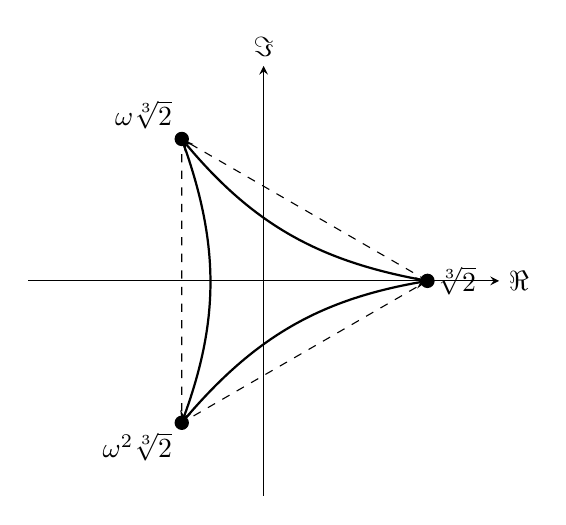
\begin{tikzpicture}[scale=1.3,>=stealth]
\draw[->] (-2.3,0)--(2.3,0) node[right]{\(\Re\)};
\draw[->] (0,-2.1)--(0,2.1) node[above]{\(\Im\)};

\coordinate (a) at (1.6,0);
\coordinate (b) at (-0.8,1.386);
\coordinate (c) at (-0.8,-1.386);

\draw[dashed] (a)--(b)--(c)--cycle;

\fill (a) circle (2pt);
\fill (b) circle (2pt);
\fill (c) circle (2pt);

\node[right] at (a) {\(\sqrt[3]{2}\)};
\node[above left] at (b) {\(\omega\sqrt[3]{2}\)};
\node[below left] at (c) {\(\omega^2\sqrt[3]{2}\)};

\draw[->,thick,bend left=20] (a) to (b);
\draw[->,thick,bend left=20] (b) to (c);
\draw[->,thick,bend left=20] (c) to (a);
\end{tikzpicture}
\end{center}

The Galois group captures algebraic permutations of these roots.

%%%%%%%%%%%%%%%%%%%%%%%%%%%%%%%%%%%%%%%%%%%%%%%%%%%%%%%%%%%%
\subsection{Roots of Unity}
\label{subsec:roots-of-unity}
%%%%%%%%%%%%%%%%%%%%%%%%%%%%%%%%%%%%%%%%%%%%%%%%%%%%%%%%%%%%

Many important Galois extensions arise from roots of

\[ x^n-1. \]

\begin{definitionbox}{Root of Unity}
An element \(\zeta\) is an \(n\)th \emph{root of unity} if
\[ \zeta^n=1. \]
\end{definitionbox}

The symbol

\[ \zeta \]

is lowercase Greek \emph{zeta}, commonly pronounced ``ZAY-tuh'' or
``ZEE-tuh.''

The complex \(n\)th roots of unity are

\[ \zeta_k=e^{2\pi ik/n},\qquad k=0,1,\ldots,n-1. \]

%%%%%%%%%%%%%%%%%%%%%%%%%%%%%%%%%%%%%%%%%%%%%%%%%%%%%%%%%%%%
\subsection{Visualizing Roots of Unity}
\label{subsec:visual-roots-unity}
%%%%%%%%%%%%%%%%%%%%%%%%%%%%%%%%%%%%%%%%%%%%%%%%%%%%%%%%%%%%

For \(n=6\), the sixth roots of unity lie equally spaced on the unit circle.

\begin{center}
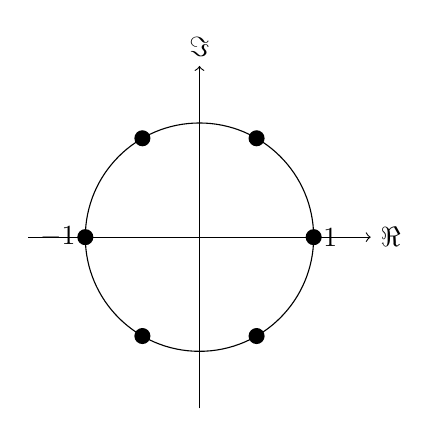
\begin{tikzpicture}[scale=1.45]
\draw[->] (-1.5,0)--(1.5,0) node[right]{\(\Re\)};
\draw[->] (0,-1.5)--(0,1.5) node[above]{\(\Im\)};
\draw (0,0) circle (1);

\foreach \k in {0,...,5}{
    \fill ({cos(60*\k)},{sin(60*\k)}) circle (2pt);
}

\node[right] at (1,0) {\(1\)};
\node[left] at (-1,0) {\(-1\)};
\end{tikzpicture}
\end{center}

Multiplication of roots of unity corresponds geometrically to adding their
angles.

%%%%%%%%%%%%%%%%%%%%%%%%%%%%%%%%%%%%%%%%%%%%%%%%%%%%%%%%%%%%
\subsection{Cyclotomic Fields}
\label{subsec:cyclotomic-fields}
%%%%%%%%%%%%%%%%%%%%%%%%%%%%%%%%%%%%%%%%%%%%%%%%%%%%%%%%%%%%

Let

\[ \zeta_n=e^{2\pi i/n} \]

be a primitive \(n\)th root of unity.

The field

\[ \Q(\zeta_n) \]

is called the \(n\)th \emph{cyclotomic field}.

The word \emph{cyclotomic} refers to division of the circle.

These fields are splitting fields of

\[ x^n-1 \]

over \(\Q\).

%%%%%%%%%%%%%%%%%%%%%%%%%%%%%%%%%%%%%%%%%%%%%%%%%%%%%%%%%%%%
\subsection{Cyclotomic Polynomials}
\label{subsec:cyclotomic-polynomials}
%%%%%%%%%%%%%%%%%%%%%%%%%%%%%%%%%%%%%%%%%%%%%%%%%%%%%%%%%%%%

\begin{definitionbox}{Cyclotomic Polynomial}
The \(n\)th \emph{cyclotomic polynomial}, denoted
\[ \Phi_n(x), \]
is the monic polynomial whose roots are exactly the primitive \(n\)th roots
of unity.
\end{definitionbox}

For example,

\[ \Phi_1(x)=x-1, \]

\[ \Phi_2(x)=x+1, \]

\[ \Phi_3(x)=x^2+x+1, \]

and

\[ \Phi_4(x)=x^2+1. \]

The notation \(\Phi_n\) uses uppercase Greek Phi and is read
``Phi sub \(n\).''

%%%%%%%%%%%%%%%%%%%%%%%%%%%%%%%%%%%%%%%%%%%%%%%%%%%%%%%%%%%%
\subsection{Euler's Totient Function and Cyclotomic Degree}
\label{subsec:cyclotomic-degree}
%%%%%%%%%%%%%%%%%%%%%%%%%%%%%%%%%%%%%%%%%%%%%%%%%%%%%%%%%%%%

The degree of \(\Phi_n(x)\) is

\[ \varphi(n), \]

where

\[ \varphi \]

is lowercase Greek \emph{phi}, pronounced ``fie'' or ``fee.''

The function

\[ \varphi(n) \]

is Euler's totient function, which counts the integers from \(1\) through
\(n\) that are relatively prime to \(n\).

Therefore,

\[ [\Q(\zeta_n):\Q]=\varphi(n). \]

Detailed study of the totient function belongs to number theory.

%%%%%%%%%%%%%%%%%%%%%%%%%%%%%%%%%%%%%%%%%%%%%%%%%%%%%%%%%%%%
\subsection{Galois Groups of Cyclotomic Fields}
\label{subsec:galois-cyclotomic-fields}
%%%%%%%%%%%%%%%%%%%%%%%%%%%%%%%%%%%%%%%%%%%%%%%%%%%%%%%%%%%%

A fundamental result states

\[ \Gal(\Q(\zeta_n)/\Q)\cong(\Z/n\Z)^\times. \]

The notation

\[ (\Z/n\Z)^\times \]

denotes the multiplicative group of invertible residue classes modulo \(n\).

Thus cyclotomic Galois groups connect field theory directly with modular
arithmetic.

%%%%%%%%%%%%%%%%%%%%%%%%%%%%%%%%%%%%%%%%%%%%%%%%%%%%%%%%%%%%
\subsection{Finite Fields and Galois Groups}
\label{subsec:galois-finite-fields}
%%%%%%%%%%%%%%%%%%%%%%%%%%%%%%%%%%%%%%%%%%%%%%%%%%%%%%%%%%%%

Consider

\[ \F_{p^n}/\F_p. \]

This is a Galois extension.

Its Galois group is generated by the Frobenius automorphism

\[ \Phi(a)=a^p. \]

Repeated application gives

\[ a\mapsto a^p\mapsto a^{p^2}\mapsto\cdots. \]

The Frobenius automorphism satisfies

\[ \Phi^n=e. \]

Therefore,

\[ \Gal(\F_{p^n}/\F_p)\cong C_n. \]

%%%%%%%%%%%%%%%%%%%%%%%%%%%%%%%%%%%%%%%%%%%%%%%%%%%%%%%%%%%%
\subsection{A Frobenius Cycle}
\label{subsec:frobenius-cycle-visual}
%%%%%%%%%%%%%%%%%%%%%%%%%%%%%%%%%%%%%%%%%%%%%%%%%%%%%%%%%%%%

\begin{center}
\begin{tikzpicture}[
    node distance=16mm,
    every node/.style={draw,rounded corners,inner sep=5pt},
    >=stealth
]
\node (a0) {\(a\)};
\node[right=of a0] (a1) {\(a^p\)};
\node[right=of a1] (a2) {\(a^{p^2}\)};
\node[right=of a2] (an) {\(a^{p^n}=a\)};

\draw[->,thick] (a0)--node[above]{\(\Phi\)}(a1);
\draw[->,thick] (a1)--node[above]{\(\Phi\)}(a2);
\draw[->,thick,dashed] (a2)--(an);
\draw[->,thick,bend right=35] (an) to node[below]{cycle} (a0);
\end{tikzpicture}
\end{center}

%%%%%%%%%%%%%%%%%%%%%%%%%%%%%%%%%%%%%%%%%%%%%%%%%%%%%%%%%%%%
\subsection{Why Galois Theory Solves Polynomial Problems}
\label{subsec:why-galois-polynomials}
%%%%%%%%%%%%%%%%%%%%%%%%%%%%%%%%%%%%%%%%%%%%%%%%%%%%%%%%%%%%

A polynomial equation may be difficult to solve directly.

Galois theory replaces the problem by studying the structure

\[ \Gal(L/K), \]

where \(L\) is the polynomial's splitting field.

Properties of this group reveal information about:

\begin{itemize}
    \item how roots are related;
    \item which intermediate fields are required;
    \item whether roots can be constructed using radicals;
    \item which symmetries must be preserved;
    \item whether certain algebraic constructions are possible.
\end{itemize}

The original equation is therefore translated into a structural group
problem.

%%%%%%%%%%%%%%%%%%%%%%%%%%%%%%%%%%%%%%%%%%%%%%%%%%%%%%%%%%%%
\subsection{Radical Extensions}
\label{subsec:radical-extensions}
%%%%%%%%%%%%%%%%%%%%%%%%%%%%%%%%%%%%%%%%%%%%%%%%%%%%%%%%%%%%

Classical formulas for quadratic, cubic, and quartic equations involve
radicals such as

\[ \sqrt{a},\qquad\sqrt[3]{a},\qquad\sqrt[4]{a}. \]

A field extension obtained through successive adjunctions of roots is called
a radical extension.

Schematically,

\[ K=K_0\subseteq K_1\subseteq\cdots\subseteq K_m, \]

where

\[ K_j=K_{j-1}(\alpha_j) \]

and

\[ \alpha_j^{n_j}\in K_{j-1}. \]

%%%%%%%%%%%%%%%%%%%%%%%%%%%%%%%%%%%%%%%%%%%%%%%%%%%%%%%%%%%%
\subsection{Solvability by Radicals}
\label{subsec:solvability-radicals}
%%%%%%%%%%%%%%%%%%%%%%%%%%%%%%%%%%%%%%%%%%%%%%%%%%%%%%%%%%%%

\begin{definitionbox}{Solvable by Radicals}
A polynomial over a field \(K\) is \emph{solvable by radicals} if its
splitting field can be contained in a field obtained from \(K\) by repeatedly
adjoining radicals.
\end{definitionbox}

The familiar quadratic formula demonstrates that every quadratic polynomial
over a characteristic-zero field is solvable by radicals.

%%%%%%%%%%%%%%%%%%%%%%%%%%%%%%%%%%%%%%%%%%%%%%%%%%%%%%%%%%%%
\subsection{Solvable Groups}
\label{subsec:galois-solvable-groups}
%%%%%%%%%%%%%%%%%%%%%%%%%%%%%%%%%%%%%%%%%%%%%%%%%%%%%%%%%%%%

Group theory contains a corresponding structural notion.

\begin{definitionbox}{Solvable Group}
A group \(G\) is \emph{solvable} if it has a finite chain of subgroups
\[ \{e\}=G_0\trianglelefteq G_1\trianglelefteq\cdots\trianglelefteq G_n=G \]
such that each quotient
\[ G_{j+1}/G_j \]
is abelian.
\end{definitionbox}

The word ``solvable'' here has a precise group-theoretic meaning.

Its importance becomes apparent through Galois theory.

%%%%%%%%%%%%%%%%%%%%%%%%%%%%%%%%%%%%%%%%%%%%%%%%%%%%%%%%%%%%
\subsection{Galois's Solvability Criterion}
\label{subsec:galois-solvability-criterion}
%%%%%%%%%%%%%%%%%%%%%%%%%%%%%%%%%%%%%%%%%%%%%%%%%%%%%%%%%%%%

\begin{theorem}[Solvability by Radicals]
Over a field of characteristic \(0\), a polynomial is solvable by radicals
if and only if its Galois group is a solvable group.
\end{theorem}

This theorem converts the question

\begin{center}
``Can the roots be expressed using radicals?''
\end{center}

into

\begin{center}
``Is the corresponding Galois group solvable?''
\end{center}

%%%%%%%%%%%%%%%%%%%%%%%%%%%%%%%%%%%%%%%%%%%%%%%%%%%%%%%%%%%%
\subsection{The Radical-Symmetry Connection}
\label{subsec:radical-symmetry-visual}
%%%%%%%%%%%%%%%%%%%%%%%%%%%%%%%%%%%%%%%%%%%%%%%%%%%%%%%%%%%%

\begin{center}
\begin{tikzpicture}[
    node distance=12mm,
    box/.style={draw,rounded corners,align=center,inner sep=6pt},
    >=stealth
]
\node[box] (poly) {Polynomial equation};
\node[box,below=of poly] (split) {Splitting field};
\node[box,below=of split] (gal) {Galois group};
\node[box,below left=of gal] (solv) {Solvable group};
\node[box,below right=of gal] (nonsolv) {Nonsolvable group};
\node[box,below=of solv] (rad) {Solvable by radicals};
\node[box,below=of nonsolv] (norad) {No radical formula};

\draw[->,thick] (poly)--(split);
\draw[->,thick] (split)--(gal);
\draw[->,thick] (gal)--(solv);
\draw[->,thick] (gal)--(nonsolv);
\draw[->,thick] (solv)--(rad);
\draw[->,thick] (nonsolv)--(norad);
\end{tikzpicture}
\end{center}

%%%%%%%%%%%%%%%%%%%%%%%%%%%%%%%%%%%%%%%%%%%%%%%%%%%%%%%%%%%%
\subsection{Why the General Quintic Has No Radical Formula}
\label{subsec:general-quintic}
%%%%%%%%%%%%%%%%%%%%%%%%%%%%%%%%%%%%%%%%%%%%%%%%%%%%%%%%%%%%

Quadratic equations possess the quadratic formula.

General cubic and quartic equations also possess formulas using radicals,
although those formulas are substantially more complicated.

A natural question is whether a similar formula exists for degree \(5\).

The answer is no.

The generic polynomial of degree \(5\) has Galois group

\[ S_5. \]

The group \(S_5\) is not solvable.

Therefore the general quintic polynomial is not solvable by radicals.

\begin{importantbox}
The Abel--Ruffini theorem does \emph{not} say that no quintic equation can be
solved by radicals.

It says there is no radical formula that solves \emph{every} quintic
equation from its coefficients in the way the quadratic formula solves every
quadratic equation.
\end{importantbox}

%%%%%%%%%%%%%%%%%%%%%%%%%%%%%%%%%%%%%%%%%%%%%%%%%%%%%%%%%%%%
\subsection{Degree Five Is the First Obstruction}
\label{subsec:degree-five-obstruction}
%%%%%%%%%%%%%%%%%%%%%%%%%%%%%%%%%%%%%%%%%%%%%%%%%%%%%%%%%%%%

The symmetric groups satisfy

\[ S_2,\quad S_3,\quad S_4 \]

are solvable, while

\[ S_n \]

is not solvable for

\[ n\geq5. \]

This group-theoretic transition explains why formulas by radicals exist in
general through degree \(4\), but fail beginning with degree \(5\).

%%%%%%%%%%%%%%%%%%%%%%%%%%%%%%%%%%%%%%%%%%%%%%%%%%%%%%%%%%%%
\subsection{Classical Geometric Constructions}
\label{subsec:galois-geometric-constructions}
%%%%%%%%%%%%%%%%%%%%%%%%%%%%%%%%%%%%%%%%%%%%%%%%%%%%%%%%%%%%

Field extensions also explain classical straightedge-and-compass
constructions.

Starting from \(\Q\), constructible numbers arise through towers of quadratic
extensions:

\[ \Q=K_0\subseteq K_1\subseteq\cdots\subseteq K_n, \]

where

\[ [K_{j+1}:K_j]=2. \]

By the Tower Law,

\[ [K_n:\Q]=2^n. \]

Thus constructibility imposes strong restrictions on possible algebraic
degrees.

%%%%%%%%%%%%%%%%%%%%%%%%%%%%%%%%%%%%%%%%%%%%%%%%%%%%%%%%%%%%
\subsection{Doubling the Cube}
\label{subsec:doubling-cube}
%%%%%%%%%%%%%%%%%%%%%%%%%%%%%%%%%%%%%%%%%%%%%%%%%%%%%%%%%%%%

Doubling a cube requires constructing

\[ \sqrt[3]{2}. \]

Its minimal polynomial over \(\Q\) is

\[ x^3-2. \]

Therefore,

\[ [\Q(\sqrt[3]{2}):\Q]=3. \]

Since \(3\) is not a power of \(2\), \(\sqrt[3]{2}\) cannot be obtained by a
tower of quadratic extensions.

Hence doubling the cube is impossible using only an unmarked straightedge
and compass.

%%%%%%%%%%%%%%%%%%%%%%%%%%%%%%%%%%%%%%%%%%%%%%%%%%%%%%%%%%%%
\subsection{Trisecting an Arbitrary Angle}
\label{subsec:angle-trisection-galois}
%%%%%%%%%%%%%%%%%%%%%%%%%%%%%%%%%%%%%%%%%%%%%%%%%%%%%%%%%%%%

Some particular angles can be trisected geometrically.

However, arbitrary angle trisection cannot always be performed with
straightedge and compass.

The obstruction can be translated into polynomial equations whose required
roots sometimes have degree not equal to a power of \(2\).

Thus field theory converts a geometric construction problem into an
algebraic degree problem.

%%%%%%%%%%%%%%%%%%%%%%%%%%%%%%%%%%%%%%%%%%%%%%%%%%%%%%%%%%%%
\subsection{Squaring the Circle}
\label{subsec:squaring-circle}
%%%%%%%%%%%%%%%%%%%%%%%%%%%%%%%%%%%%%%%%%%%%%%%%%%%%%%%%%%%%

Squaring the circle would require constructing a square with the same area as
a given circle.

For a unit circle, the required side length is

\[ \sqrt{\pi}. \]

Since \(\pi\) is transcendental over \(\Q\), it cannot arise from any finite
tower of algebraic quadratic extensions.

Therefore squaring the circle is impossible using only straightedge and
compass.

%%%%%%%%%%%%%%%%%%%%%%%%%%%%%%%%%%%%%%%%%%%%%%%%%%%%%%%%%%%%
\subsection{A Structural View of Classical Problems}
\label{subsec:classical-problems-visual}
%%%%%%%%%%%%%%%%%%%%%%%%%%%%%%%%%%%%%%%%%%%%%%%%%%%%%%%%%%%%

\begin{center}
\begin{tikzpicture}[
    node distance=10mm,
    box/.style={draw,rounded corners,align=center,inner sep=5pt,font=\small},
    >=stealth
]
\node[box] (geo) {Geometric construction};
\node[box,below=of geo] (num) {Required number};
\node[box,below=of num] (poly) {Polynomial / field extension};
\node[box,below=of poly] (degree) {Extension degree};
\node[box,below=of degree] (test) {Power of \(2\)?};

\draw[->,thick] (geo)--(num);
\draw[->,thick] (num)--(poly);
\draw[->,thick] (poly)--(degree);
\draw[->,thick] (degree)--(test);
\end{tikzpicture}
\end{center}

This is an example of the broader algebraic philosophy: translate a problem
into structure, then use structural invariants to determine what is possible.

%%%%%%%%%%%%%%%%%%%%%%%%%%%%%%%%%%%%%%%%%%%%%%%%%%%%%%%%%%%%
\subsection{Common Errors in Galois Theory}
\label{subsec:common-galois-errors}
%%%%%%%%%%%%%%%%%%%%%%%%%%%%%%%%%%%%%%%%%%%%%%%%%%%%%%%%%%%%

\subsubsection{Assuming Every Field Extension Is Galois}

A field extension must satisfy additional conditions.

For finite extensions,

\[ \text{Galois}=\text{normal}+\text{separable}. \]

For example,

\[ \Q(\sqrt[3]{2})/\Q \]

is not Galois.

%%%%%%%%%%%%%%%%%%%%%%%%%%%%%%%%%%%%%%%%%%%%%%%%%%%%%%%%%%%%
\subsubsection{Assuming the Galois Group Is Always \(S_n\)}

If a polynomial has degree \(n\), its Galois group can often be represented
as a subgroup of \(S_n\), but it need not equal all of \(S_n\).

For example,

\[ \Gal(\Q(\sqrt2)/\Q)\cong C_2. \]

%%%%%%%%%%%%%%%%%%%%%%%%%%%%%%%%%%%%%%%%%%%%%%%%%%%%%%%%%%%%
\subsubsection{Forgetting Which Field Is Fixed}

The notation

\[ \Gal(L/K) \]

specifically means automorphisms of \(L\) that fix \(K\).

Changing the base field may change the Galois group.

%%%%%%%%%%%%%%%%%%%%%%%%%%%%%%%%%%%%%%%%%%%%%%%%%%%%%%%%%%%%
\subsubsection{Forgetting Inclusion Reversal}

Under the Galois correspondence,

\[ E_1\subseteq E_2 \]

corresponds to

\[ \Gal(L/E_2)\leq\Gal(L/E_1). \]

Larger fields correspond to smaller groups.

%%%%%%%%%%%%%%%%%%%%%%%%%%%%%%%%%%%%%%%%%%%%%%%%%%%%%%%%%%%%
\subsubsection{Confusing Normal Extensions with Normal Subgroups}

These are related but distinct concepts.

A normal extension is a field-theoretic property.

A normal subgroup is a group-theoretic property.

The Fundamental Theorem of Galois Theory connects them.

%%%%%%%%%%%%%%%%%%%%%%%%%%%%%%%%%%%%%%%%%%%%%%%%%%%%%%%%%%%%
\subsubsection{Assuming Solvable Group Means Easy to Solve}

A solvable group is defined through a chain of normal subgroups with abelian
quotients.

The term does not mean that computations involving the group are necessarily
easy.

%%%%%%%%%%%%%%%%%%%%%%%%%%%%%%%%%%%%%%%%%%%%%%%%%%%%%%%%%%%%
\subsubsection{Misinterpreting the Abel--Ruffini Theorem}

The theorem does not say that quintic equations never have radical solutions.

Some quintics do.

The theorem says that no universal formula by radicals exists for all
quintic equations.

%%%%%%%%%%%%%%%%%%%%%%%%%%%%%%%%%%%%%%%%%%%%%%%%%%%%%%%%%%%%
\subsection{Applications of Galois Theory}
\label{subsec:galois-applications}
%%%%%%%%%%%%%%%%%%%%%%%%%%%%%%%%%%%%%%%%%%%%%%%%%%%%%%%%%%%%

\begin{applicationbox}
\textbf{Polynomial Equations.}
Galois groups determine structural relationships among polynomial roots and
whether equations are solvable by radicals.

\medskip

\textbf{Field Theory.}
Galois theory organizes intermediate fields through subgroup structure and
explains normal and separable extensions.

\medskip

\textbf{Group Theory.}
Permutation groups, normal subgroups, quotient groups, and solvable groups
receive direct interpretations through polynomial equations.

\medskip

\textbf{Number Theory.}
Cyclotomic fields, algebraic number fields, finite fields, and arithmetic
extensions are central objects in modern number theory.

\medskip

\textbf{Geometry.}
Field extensions explain classical straightedge-and-compass construction
problems.

\medskip

\textbf{Finite Fields.}
The Galois groups of finite fields are generated by Frobenius automorphisms
and play important roles in coding theory and arithmetic.

\medskip

\textbf{Algebraic Geometry.}
Extensions of fields and their automorphisms are fundamental when studying
algebraic varieties over different base fields.

\medskip

\textbf{Modern Algebra.}
Galois theory is one of the clearest examples of how apparently different
mathematical structures can encode the same information.
\end{applicationbox}

%%%%%%%%%%%%%%%%%%%%%%%%%%%%%%%%%%%%%%%%%%%%%%%%%%%%%%%%%%%%
\subsection{Structural Map of Galois Theory}
\label{subsec:galois-structural-map}
%%%%%%%%%%%%%%%%%%%%%%%%%%%%%%%%%%%%%%%%%%%%%%%%%%%%%%%%%%%%

\begin{center}
\begin{tikzpicture}[
    node distance=9mm and 14mm,
    box/.style={draw,rounded corners,align=center,inner sep=4pt,font=\small},
    >=stealth
]
\node[box] (poly) {Polynomial};
\node[box,below=of poly] (split) {Splitting field};
\node[box,below=of split] (galext) {Galois extension};
\node[box,below=of galext] (group) {Galois group};

\node[box,below left=of group] (sub) {Subgroups};
\node[box,below right=of group] (normal) {Normal subgroups};

\node[box,below=of sub] (fields) {Intermediate fields};
\node[box,below=of normal] (gfields) {Galois intermediate\\extensions};

\node[box,below left=of fields] (rad) {Radicals};
\node[box,below right=of gfields] (geom) {Constructibility};

\draw[->] (poly)--(split);
\draw[->] (split)--(galext);
\draw[->] (galext)--(group);
\draw[->] (group)--(sub);
\draw[->] (group)--(normal);
\draw[->] (sub)--(fields);
\draw[->] (normal)--(gfields);
\draw[->] (fields)--(rad);
\draw[->] (gfields)--(geom);
\end{tikzpicture}
\end{center}

%%%%%%%%%%%%%%%%%%%%%%%%%%%%%%%%%%%%%%%%%%%%%%%%%%%%%%%%%%%%
\subsection{Exercises}
\label{subsec:galois-theory-exercises}
%%%%%%%%%%%%%%%%%%%%%%%%%%%%%%%%%%%%%%%%%%%%%%%%%%%%%%%%%%%%

\begin{exercise}[1]
Define \(\Gal(L/K)\) in words.
\end{exercise}

\begin{exercise}[1]
What does it mean for an automorphism of \(L\) to fix \(K\)?
\end{exercise}

\begin{exercise}[1]
Determine
\[ \Gal(\Q(\sqrt3)/\Q). \]
\end{exercise}

\begin{exercise}[1]
Determine
\[ \Gal(\Q(i)/\Q). \]
\end{exercise}

\begin{exercise}[2]
Show that
\[ \Gal(\Q(\sqrt5)/\Q)\cong C_2. \]
\end{exercise}

\begin{exercise}[2]
Prove that a \(K\)-automorphism sends a root of a polynomial in \(K[x]\) to
another root of the same polynomial.
\end{exercise}

\begin{exercise}[1]
Find the conjugates of \(\sqrt7\) over \(\Q\).
\end{exercise}

\begin{exercise}[1]
Find the conjugates of \(i\) over \(\R\).
\end{exercise}

\begin{exercise}[2]
Determine whether
\[ x^3-5 \]
is separable over \(\Q\).
\end{exercise}

\begin{exercise}[2]
Determine whether
\[ x^4-2 \]
is separable over \(\Q\).
\end{exercise}

\begin{exercise}[2]
Explain why every irreducible polynomial over \(\Q\) is separable.
\end{exercise}

\begin{exercise}[2]
Explain why finite fields are perfect.
\end{exercise}

\begin{exercise}[2]
Determine whether
\[ \Q(\sqrt2)/\Q \]
is normal.
\end{exercise}

\begin{exercise}[2]
Determine whether
\[ \Q(\sqrt[3]{2})/\Q \]
is normal.
\end{exercise}

\begin{exercise}[2]
Find the splitting field of
\[ x^3-2 \]
over \(\Q\).
\end{exercise}

\begin{exercise}[2]
Explain why
\[ \C/\R \]
is Galois.
\end{exercise}

\begin{exercise}[2]
Verify that
\[ |\Gal(\C/\R)|=[\C:\R]. \]
\end{exercise}

\begin{exercise}[2]
Let
\[ G=\Gal(\Q(\sqrt2)/\Q). \]
Find the fixed field of \(G\).
\end{exercise}

\begin{exercise}[2]
Let complex conjugation act on \(\C\). Prove that its fixed field is \(\R\).
\end{exercise}

\begin{exercise}[2]
State the Fundamental Theorem of Galois Theory in your own words.
\end{exercise}

\begin{exercise}[2]
Explain why inclusion is reversed in the Galois correspondence.
\end{exercise}

\begin{exercise}[2]
Suppose \(L/K\) is finite Galois with
\[ |\Gal(L/K)|=12. \]
If \(H\leq\Gal(L/K)\) has order \(3\), find
\[ [L:L^H] \]
and
\[ [L^H:K]. \]
\end{exercise}

\begin{exercise}[2]
Suppose
\[ [L:K]=8 \]
and \(L/K\) is Galois. What is the order of \(\Gal(L/K)\)?
\end{exercise}

\begin{exercise}[2]
For
\[ L=\Q(\sqrt2,\sqrt3), \]
verify that
\[ [L:\Q]=4. \]
\end{exercise}

\begin{exercise}[2]
List the four automorphisms of
\[ \Q(\sqrt2,\sqrt3)/\Q. \]
\end{exercise}

\begin{exercise}[3]
Construct the multiplication table for
\[ \Gal(\Q(\sqrt2,\sqrt3)/\Q). \]
Identify the group.
\end{exercise}

\begin{exercise}[3]
Find the subgroup fixing
\[ \Q(\sqrt2) \]
inside
\[ \Gal(\Q(\sqrt2,\sqrt3)/\Q). \]
\end{exercise}

\begin{exercise}[3]
Find the subgroup fixing
\[ \Q(\sqrt6). \]
\end{exercise}

\begin{exercise}[3]
Draw the complete field lattice and subgroup lattice for
\[ \Q(\sqrt2,\sqrt3)/\Q. \]
\end{exercise}

\begin{exercise}[2]
Explain the significance of a normal subgroup under the Galois
correspondence.
\end{exercise}

\begin{exercise}[2]
Suppose
\[ H\trianglelefteq G=\Gal(L/K). \]
Explain the relationship between \(G/H\) and the corresponding intermediate
field.
\end{exercise}

\begin{exercise}[2]
Find the roots of unity satisfying
\[ z^4=1. \]
Plot them on the complex plane.
\end{exercise}

\begin{exercise}[2]
Find the roots of unity satisfying
\[ z^3=1. \]
\end{exercise}

\begin{exercise}[2]
Determine
\[ \Phi_5(x). \]
\end{exercise}

\begin{exercise}[2]
Compute
\[ \varphi(8). \]
Hence determine
\[ [\Q(\zeta_8):\Q]. \]
\end{exercise}

\begin{exercise}[3]
Determine
\[ \Gal(\Q(\zeta_5)/\Q) \]
up to isomorphism.
\end{exercise}

\begin{exercise}[2]
Determine
\[ \Gal(\F_{2^3}/\F_2). \]
\end{exercise}

\begin{exercise}[2]
Determine
\[ \Gal(\F_{5^4}/\F_5). \]
\end{exercise}

\begin{exercise}[3]
Show that the Frobenius automorphism generates
\[ \Gal(\F_{p^n}/\F_p). \]
\end{exercise}

\begin{exercise}[2]
Explain what it means for a polynomial to be solvable by radicals.
\end{exercise}

\begin{exercise}[2]
Explain the difference between a solvable equation and a solvable group.
\end{exercise}

\begin{exercise}[2]
Why does the nonsolvability of \(S_5\) matter for quintic equations?
\end{exercise}

\begin{exercise}[2]
Explain why the Abel--Ruffini theorem does not imply that every quintic is
impossible to solve by radicals.
\end{exercise}

\begin{exercise}[2]
Explain why constructible numbers must lie in extensions whose degree over
\(\Q\) is a power of \(2\).
\end{exercise}

\begin{exercise}[2]
Use field degrees to explain why doubling the cube is impossible by
straightedge and compass.
\end{exercise}

\begin{exercise}[3]
Research within the later geometry chapters of this text how field extensions
connect to constructible regular polygons.
\end{exercise}

%%%%%%%%%%%%%%%%%%%%%%%%%%%%%%%%%%%%%%%%%%%%%%%%%%%%%%%%%%%%
\subsection{Section Connections}
\label{subsec:galois-theory-connections}
%%%%%%%%%%%%%%%%%%%%%%%%%%%%%%%%%%%%%%%%%%%%%%%%%%%%%%%%%%%%

\chapterconnection{
Galois theory unifies several major ideas developed throughout algebra.
Polynomial rings and irreducibility from \cref{sec:ring-theory} determine
algebraic extensions and splitting fields from \cref{sec:field-theory}.
Automorphisms of those fields form groups governed by the theory developed in
\cref{sec:group-theory}. The Fundamental Theorem of Galois Theory then
establishes a correspondence between intermediate fields and subgroups,
turning questions about polynomial roots into questions about group
structure. These ideas lead naturally into algebraic number theory,
cyclotomic theory, finite fields, algebraic geometry, and deeper forms of
representation and structural algebra.
}

%%%%%%%%%%%%%%%%%%%%%%%%%%%%%%%%%%%%%%%%%%%%%%%%%%%%%%%%%%%%
% SECTION SOURCE TRACKING
%%%%%%%%%%%%%%%%%%%%%%%%%%%%%%%%%%%%%%%%%%%%%%%%%%%%%%%%%%%%

%------------------------------------------------------------
% 1.7 Galois Theory
%------------------------------------------------------------
%
% Sources:
%   - Thomas W. Judson, Abstract Algebra: Theory and Applications.
%     Key: judson2025abstractalgebra
%
% Used for:
%   - field automorphisms and Galois groups;
%   - root permutations and conjugates;
%   - separable and normal extensions;
%   - finite Galois extensions;
%   - fixed fields and intermediate fields;
%   - Fundamental Theorem of Galois Theory;
%   - subgroup-field correspondence;
%   - cyclotomic and finite-field examples;
%   - solvability by radicals and classical applications.
%
% Notes:
%   - Group-theoretic foundations are treated canonically in Section 1.4.
%   - Ring and polynomial foundations are treated canonically in Section 1.5.
%   - Field extensions, minimal polynomials, splitting fields, and finite-field
%     foundations are treated canonically in Section 1.6.
%   - This section focuses on the structural correspondence between field
%     extensions and groups rather than repeating those prerequisite theories.
%   - Advanced topics such as infinite Galois theory, profinite groups,
%     Galois cohomology, inverse Galois theory, and differential Galois theory
%     belong to later specialized study.
%   - Visualizations and exposition are independently developed for this text.
%
\nocite{judson2025abstractalgebra}